\chapter{Tecnica Ottimizzata}

In questo capitolo viene presentata un'ottimizzazione al problema descritto nel capitolo precedente.
Tale ottimizzazione si basa sul principio della decomposizione bilanciata.
Si fa vedere, inoltre, come l'utilizzo di quest'ultima permetta un notevole miglioramento delle performance.

\section{Decomposizioni Bilanciate di un albero}
Si vuole andare a dimostrare in questo paragrafo, che dato un albero T \`e sempre possibile ricavare una scomposizione bilanciata dell'albero.
\\
Prima di poter enunciare il teorema e dimostrarlo occorre dare delle nozioni preliminari.

\newtheorem{definizione}{Definizione}[section]
\newtheorem{lemma}[definizione]{Lemma}
\begin{definizione}
	\label{definizioneDeco}
Sia $T_r$ un albero radicato nel nodo r , con k nodi.
Diremo che la coppia (A,B), dove  A e B sono insiemi contenenti i nodi di $T_r$, \`e una decomposizione per l'albero se:
\begin{itemize}
	\item $| A |\cup| B | = k$
	\item $A \cap B = r$.
\end{itemize}
\end{definizione}


\begin{lemma}
\label{lemmaDeco}
Dato un albero $ T $, e una sua decomposizione $ (A,B) $, affinch\`e tale decomposizione sia bilanciata dovr\`a risultare che:
\begin{equation*}
	\max{ \{|A| , |B| \} }  \le  f(k)
\end{equation*}


dove f(k) \`e il fattore di bilanciamento, varia in funzione al numero dei nodi dell'albero ed \`e pari a:
\begin{equation*}
f(k) = \left\lceil \frac{2}{3}  k  \right\rceil + 1
\end{equation*}
\end{lemma}\mbox{}

\begin{proof}
Per dimostrare il lemma si fa una dimostrazione costruttiva, mediante il seguente algoritmo.
In input si ha, un albero $ T $ e due insiemi di nodi $ A $ e $ B $ entrambi inizialmente vuoti.
Per prima cosa si inserisce la radice in entrambi gli insiemi.
Si supponga, che il numero dei sottoalberi radicati nella radice di $ T $ sia $ i \ge 2 $, perch\`e altrimenti verrebbe subito meno la Definizione \ref{definizioneDeco} , e che i $ T_i $ sottoalberi siano ordinati per dimensione, in ordine non crescente.
Per prima cosa si calcola il valore di $ f(k) $ applicato ai nodi dell'albero $ T $.
Il primo passo inserisce in $ A $ i nodi di $ T_1 $.
Il secondo prova ad aggiunge ad $ A $ i nodi di $ T_2 $.
Se $ |A| + |T_2| \le f(k) $ allora aggiorna $ A $ inserendo i nodi di $ T_2 $ e ripete il passo due su $ T_3 $, altrimenti l'algoritmo si arresta inserendo tutti i nodi dei sottoalberi rimanenti in $ B $.
In realt\'a una volta trovato un $ T_i $ che non pu\`o essere aggiunto ad $ A $ l'algoritmo potrebbe continuare a vedere i sottoalberi a seguire, ma in questo caso si suppone che l'algoritmo si arresti.
\end{proof}

Come si pu\`o capire dalla dimostrazione del Lemma \ref{lemmaDeco}, le decomposizioni bilanciate cos\`i come sono definite fino ad ora non possono essere applicate su tutti gli alberi, ma solo su alcuni.
Occorrono, perci\`o ulteriori definizioni.
   
\begin{definizione}
Per ogni nodo v di un albero T, le diramazioni di T  rispetto a v, sono tutti i sottoalberi massimali, radicati nei figli di v. 
Sia $\alpha(v)$ il numero di nodi della massima diramazione di v. 

Un nodo u di un albero T con n nodi, \`e un nodo centroide se $\alpha(u)\le\frac{n}{2}$.

Il centroide di un albero non \`e necessariamente unico, infatti Jordan \cite{jordan1869assemblages}  ha dimostrato che o (i) T ha un singolo centroide v e $\alpha(v) < \frac{n}{2}$ oppure (ii) t ha due nodi centroidi (adiacenti) $v_1$ e $v_2$ tali che $\alpha(v_1) = \alpha(v_2) = \frac{n}{2}$, in questo caso il numero di nodi n \`e pari.
\end{definizione}

Esistono diversi algoritmi per la ricerca del centroide, quello da noi usato \`e l'algoritmo di Jordan che  ha una complessit\`a temporale lineare al numero di nodi O(n). \\
Il primo passo da fare \`e determinare $\alpha(v)$ $\forall v \in T$.\\
Per poter calcolare $\alpha$ $\forall v \in T$, inizialmente si effettua una visita DFS (Depth First Search) dell'albero a partire dalla radice, in modo da definire la cardinalit\`a di ogni possibile sottoalbero a partire dalla radice, procedendo su ogni suo figlio .
I sottoalberi ottenuti dai nodi foglia e dal nodo radice, sono alberi banali che avranno rispettivamente cardinalit\`a 1 e $|T|$. \\
A questo punto si pu\`o procedere con l'individuazione di $\alpha (v)$, ossia $\forall v$ della diramazione con un maggior numero di nodi.

Per farlo, si considera ogni nodo v di T e si calcola la cardinalit\`a dei sottoalberi radicati in ognuna delle sue possibili diramazioni. 
$\alpha (v)$ sar\`a il valore massimo tra tutte le quantit\`a individuate.
\\

\paragraph{Esempio 1}\mbox{}\\
Si prenda l'albero T in figura \ref{fig:1}.\\ 
T ha otto nodi e per ogni nodo \`e indicata la cardinalit\`a del sottoalbero radicato in esso.
	\begin{figure}[htbp]
	\centering
	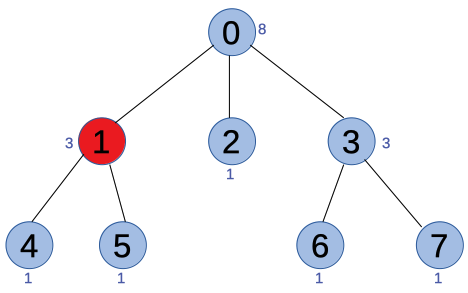
\includegraphics[width=10cm]{capitolo3/1}
	\caption{}
	\label{fig:1}
\end{figure}
Perci\`o per il nodo {\color{red} 1}, si avr\`a che:
\begin{equation*}
\alpha(1) = max {\{ |T_4| , |T_5| , (|T| - |T_1| )\}} = \max{\{1, 1, 5\} }  = 5
\end{equation*}
Dove $T_4$ rappresenta il sottoalbero di T radicato nel nodo 4, analogamente $ T_5 $, mentre con l'ultimo valore rappresentiamo la cardinalit\`a del sottoalbero radicato in 0, che conterr\'a tutti i nodi restanti non inclusi nel sottoalbero di T radicato in 1. 
\mbox{}\\\\
Una volta determinato $\alpha(v)$ $\forall v \in T$, si procede alla ricerca del centroide, che sar\`a il nodo di T per cui vale la seguente disuguaglianza:
\begin{equation*}
\alpha(v) \le \left\lfloor\frac{n}{2} \right\rfloor
\end{equation*}
	\begin{figure}[!htb]
	\begin{minipage}{0.48\textwidth}
		\centering
		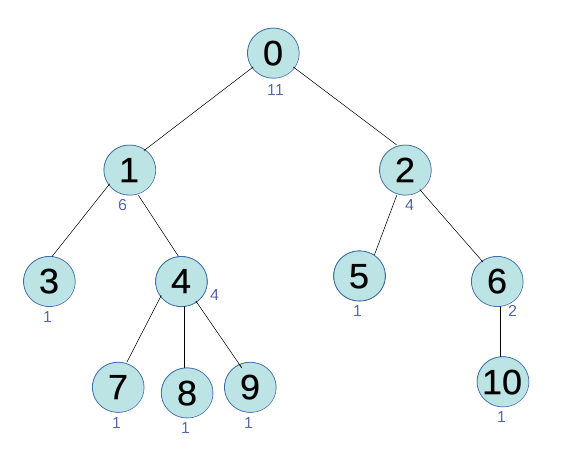
\includegraphics[width=5.26cm]{capitolo3/grafo1c}
		\caption{Rappresentazione dell'albero T}
		\label{fig:2}
	\end{minipage}\hfill
	\begin{minipage}{0.48\textwidth}
		\centering
		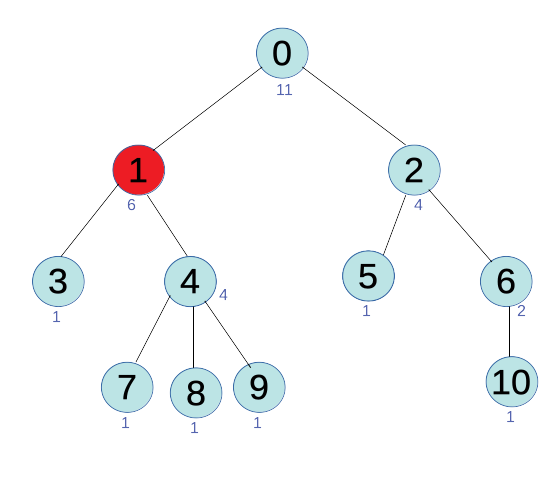
\includegraphics[width=5.8cm]{capitolo3/grafo2}
		\caption{Rappresentazione del centroide in T}
		\label{fig:3}
	\end{minipage}7
\end{figure}
\mbox{}\\\\
\paragraph{Esempio 2}\mbox{}\\
Si consideri l'albero T in figura \ref{fig:2} per la ricerca del nodo centroide.
Per prima cosa  viene calcolato $\alpha(v)$ su ogni nodo di T, numerati da 0 a 10. \\
Quello che si otterr\`a sar\`a:

%$\alpha(0) = 6$; $\alpha(1) = 5$; $\alpha(2) = 7$; $\alpha(3) = 10$; $\alpha(4) = 7$; $\alpha(5) =  10$ $\alpha(6) = 9$; $\alpha(7) = 10$; $\alpha(8) = 10$; $\alpha(9) = 10$; $\alpha(10) = 10$.


\begin{center}
	\begin{tabular}{ c c c c c  }
		$\alpha(0) = 6$ & & $\alpha(1) = 5$ & & $\alpha(2) = 7$ \\ 
		$\alpha(3) = 10$ && $\alpha(4) = 7$ &&  $\alpha(5) =  10$ \\  
		$\alpha(6) = 9$ && $\alpha(7) = 10$ && $\alpha(8) = 10$ \\
		 $\alpha(9) = 10$ && $\alpha(10) = 10$ &&
	\end{tabular}
\end{center}

Poich\'e $ \left\lfloor\frac{n}{2} \right\rfloor = \left\lfloor \frac{11}{2} \right\rfloor = 5$, basta verificare per quale nodo v di T , vale che $\alpha(v) \le \left\lfloor\frac{n}{2} \right\rfloor$.
L'unico nodo per cui tale disuguaglianza risulta vera \`e il nodo 1, infatti $5\le 5$, e sar\`a l'unico centroide dell'albero T (figura \ref{fig:3}).


Come gi\'a accennato l'algoritmo ha complessit\`a lineare sul numero dei nodi.
Infatti, occorre calcolare il grado di ogni nodo e successivamente verificare che ci siano le condizioni affich\`e risulti un centroide e si ha:

\begin{equation*}
\sum_{v}^{}(1 + \delta(v)) = n + \sum_{v}^{} \delta(v) = n+n-1= 2n-1 =O(n)
\end{equation*}\\
In base a tutte le nozioni illustrate in precedenza possiamo passare a ad enunciare il  teorema di seguito.

\paragraph{Teorema}\mbox{}\\
Per ogni albero T di k nodi esiste un nodo r di T , tale che l’albero $T_r$, ottenuto radicando T in r ammette una decomposizione bilanciata.

\paragraph{Dimostrazione}\mbox{}\\
Sia un albero T con pi\`u di due nodi(per $n\le2$ caso banale). \\
La prima operazione da compiere \`e l’individuazione del nodo r di T, su cui si andr\`a poi a radicare l’albero.
Banalmente, per come \`e stato definito, il nodo che si cerca, non \`e altro che  un centroide dell’albero T, quindi si applica l’algoritmo precedentemente descritto per la sua ricerca.
Una volta trovato, questo sar\`a il nuovo nodo su cui sar\`a radicato l’albero T, che da questo punto sar\`a indicato con $T_r$.
\\ 
Inoltre supponiamo, senza perdere di generalit\`a, che i sottoalberi radicati nei figli di r siano ordinati in maniera non crescente rispetto alla loro dimensione.\\
\`E possibile ottenere una scomposizione, (A,B), dei k nodi di $T_r$,  tale che un insieme, ad esempio A, contenga al massimo i $\left\lceil \frac{2}{3} \right\rceil$ dei nodi dell’albero e B il restante di essi.\\
Ovviamente questo algoritmo terminer\`a, poich\'e il numero di nodi \`e finito.
Inoltre l’insieme con il maggior numero di elementi non conterr\`a pi\`u dei $\left\lceil \frac{2}{3} \right\rceil$ del totale. \\
Per dimostrarlo si osserver\`a che A deve contenere almeno $\frac{1}{3}$ dei nodi totali. \\
Si suppone di aver inserito nell’insieme A una certa quantit\`a di elementi, sia un numero pari a $\frac{2}{3}$k. \\
Sia x il primo elemento non in A e sia i la sua posizione (figura \ref{fig:4}).
	\begin{figure}[htbp]
	\centering
	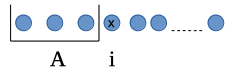
\includegraphics[width=6cm]{capitolo3/3}
	\caption{}
	\label{fig:4}
\end{figure}

Si possono verificare  due casi:
\begin{itemize}
	\item (i=2)  L’insieme A \`e formato da un unico elemento y:
		\begin{figure*}[htbp]
		\centering
		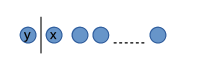
\includegraphics[width=6cm]{capitolo3/4}
			\caption{}
	\end{figure*}\\
Per come \`e costruzione di A, si avr\`a certamente che:
\\
\begin{equation}
 y + x > \frac{2}{3}k
\end{equation}
\\
Dividendo entrambi i membri di (1) per  due, si ottiene:
\\
\begin{equation}
\frac{ x + y }{2} > \frac{k}{3}  
\end{equation}
Si nota che $\frac{ x + y }{2} $ rappresenta esattamente il valore medio. \\
Dall’ordinamento dei sottoalberi di $T_r$, risulta che $y \ge x$ perci\`o si avr\`a che:
\begin{equation}
y \ge \frac{ x + y }{2} 
\end{equation}
unendo la (2) e la (3)  si ottiene:
\begin{equation*}
y > \frac{k}{3}  
\end{equation*}
\item ($i\ge3$) In A vi sono almeno due elementi. Sia s il valore ottenuto dalla loro somma 
	\begin{figure*}[htbp]
	\centering
	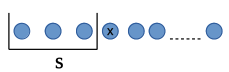
\includegraphics[width=6cm]{capitolo3/5}
		\caption{}
\end{figure*}\\
Si avr\`a che:
\begin{equation}
s+ x > \frac{2}{3}
\end{equation}
Inoltre, per costruzione:
\begin{equation}
x \le \frac{k}{3}
\end{equation}
Sottraendo la (5) alla (4), ammissibile poich\'e rispetta le regole delle disequazioni, si otterr\`a:\\
\begin{equation}
	s + x - x > \frac{2}{3} k - \frac{k}{3} \hspace{0.3cm} \text{    ossia    }\hspace{0.3cm} s > \frac{k}{3}
\end{equation}
Perci\`o gli insiemi ottenuti dalla scomposizione di $T_r$ avranno cardinalit\`a compresa tra $\frac{1}{3} k$ e $\frac{2}{3} k$, garantendo cos\`i delle decomposizioni bilanciate.\\ 
Nel caso in cui si abbiano due centroidi, la scelta su quale radicare l’albero  \`e deterministica e  viene fatta prendendo quello che, tra i due, ha un $k(v)$ minore rispetto alla relazione d’ordine precedentemente fornita.


\end{itemize}

